\whiteBGstarBegin
\setcounter{section}{0}
\section{Từ thông. Cảm ứng điện từ}
\begin{enumerate}[label=\bfseries Câu \arabic*:]
	
	\item \mkstar{2} 
	
	\cauhoi{
		
			Mạch kín tròn (C) nằm trong cùng mặt phẳng P với dòng điện thẳng $I$. Hỏi trường hợp nào dưới đây, từ thông qua (C) biến thiên?
		\begin{center}
			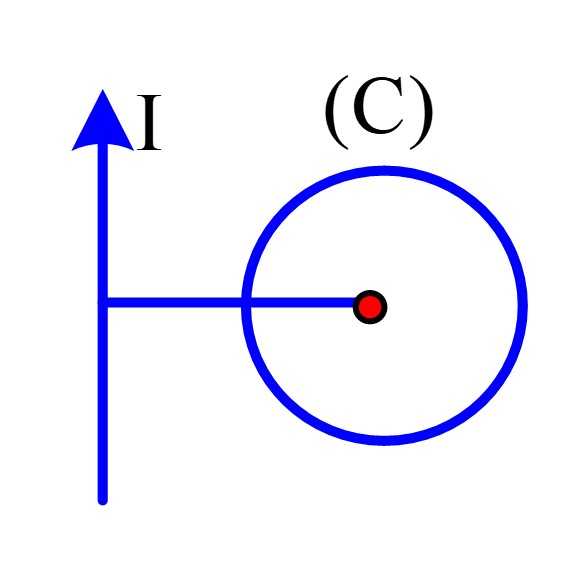
\includegraphics[scale=0.2]{../figs/VN11-PH-29-P-0191-1}
		\end{center}
		\begin{mcq}(1)
			\item{(C) dịch chuyển trong mặt phẳng P lại gần $I$ hoặc ra xa $I$.}
			\item{(C) dịch chuyển trong mặt phẳng P với vận tốc song song với dòng $I$.}
			\item{(C) cố định, dây dẫn thẳng mang dòng $I$ chuyển động tịnh tiến dọc theo chính nó.}
			\item{(C) quay xung quanh dòng điện thẳng $I$.}
		\end{mcq}
	}
	
	\loigiai{
		\textbf{Đáp án: A.}
		
		Vì từ trường của dòng điện thẳng I mạnh ở những điểm gần dòng điện và càng giảm ở những điểm càng xa dòng điện.
		
		Suy ra trường hợp (C) dịch chuyển trong P lại gần I hoặc ra xa I thì từ thông qua (C) biến thiên.
	}
	
	\item \mkstar{2} 
	
	\cauhoi{
	Cho một nam châm thẳng rơi theo phương thẳng đứng qua tâm $\text O$ của vòng dây dẫn tròn nằm ngang như hình vẽ. Trong quá trình nam châm rơi, vòng dây xuất hiện dòng điện cảm ứng có chiều
	\begin{center}
		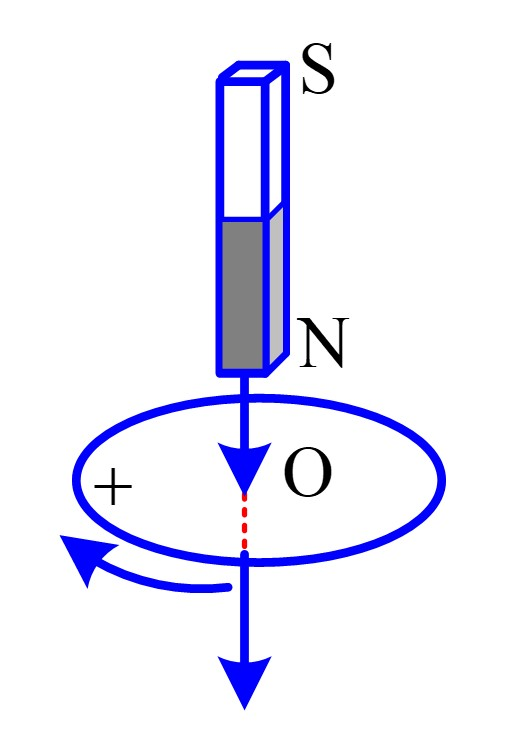
\includegraphics[scale=0.25]{../figs/VN11-PH-29-P-0191-2}
	\end{center}
	\begin{mcq}(1)
		\item là chiều dương quy ước trên hình.
		\item ngược với chiều dương quy ước trên hình.
		\item ngược với chiều dương quy ước khi nam châm ở phía trên vòng dây và chiều ngược lại khi nam châm ở phía dưới.
		\item là chiều dương quy ước khi nam châm ở phía trên vòng dây và chiều ngược lại khi nam châm ở phía dưới.
	\end{mcq}
		
	}
	
	\loigiai{
		\textbf{Đáp án: C.}
		

	}
	
	\item \mkstar{2} 
	
	\cauhoi{
		Chiều dòng điện cảm ứng trong vòng dây đúng là
		\begin{center}
			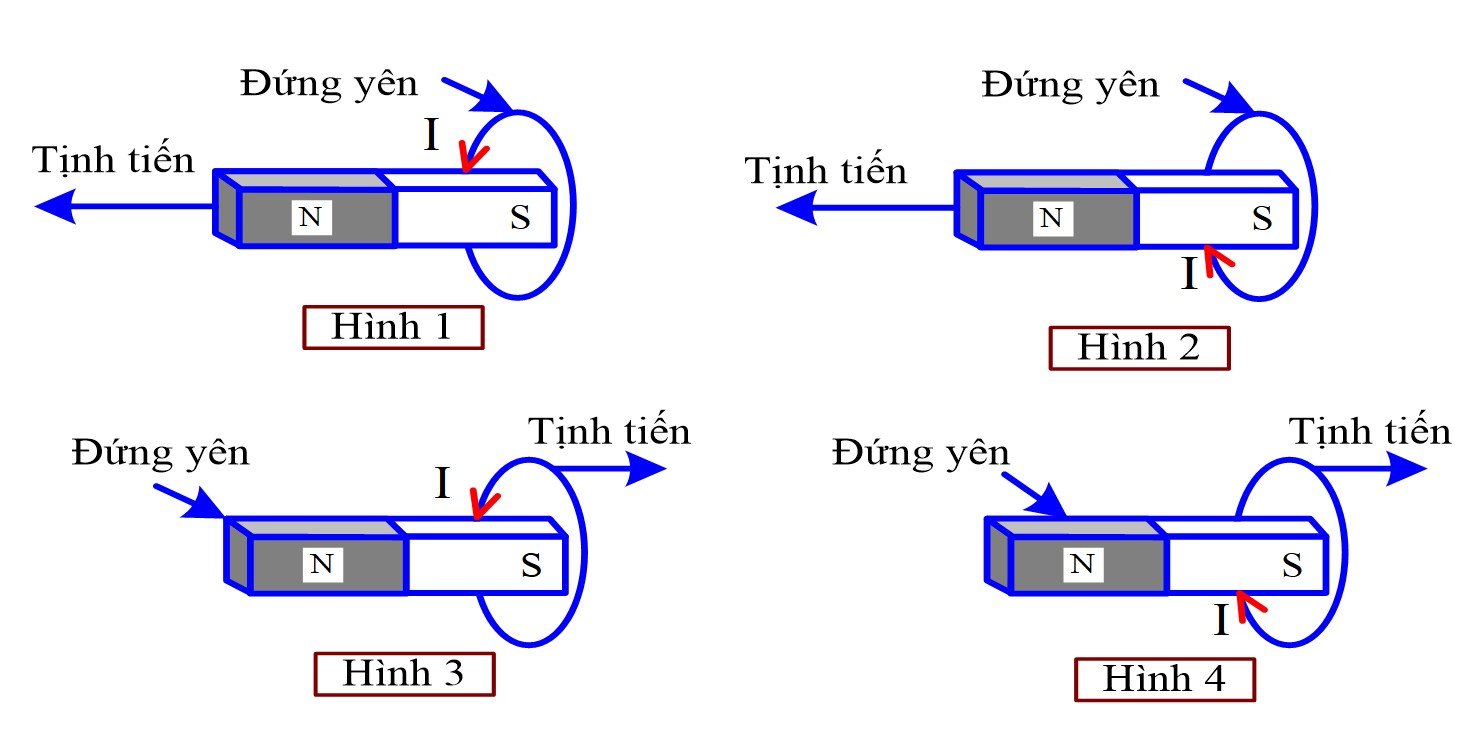
\includegraphics[scale=0.4]{../figs/VN11-PH-29-P-0191-3}
		\end{center}
		\begin{mcq}(2)
			\item{Hình 1 và Hình 2.}
			\item{Hình 1 và Hình 3.}
			\item{Hình 2 và Hình 4.}
			\item{Hình 4 và Hình 3.}
		\end{mcq}
	}
	
	\loigiai{
		\textbf{Đáp án: B.}
		
		
	}
	\item \mkstar{2} 
	
	\cauhoi{
		Một thanh nam châm NS được đặt thẳng đứng song song với mặt phẳng chứa vòng dây dẫn (C) và có trục quay O vuông góc với trục của vòng dây, chiều dương trên vòng dây được chọn như hình vẽ. Thanh nam châm NS chuyển động quay góc $\ang{90}$ để cực Nam (S) của nó tới đối diện với vòng dây dẫn (C) thì trong (C)
		\begin{center}
			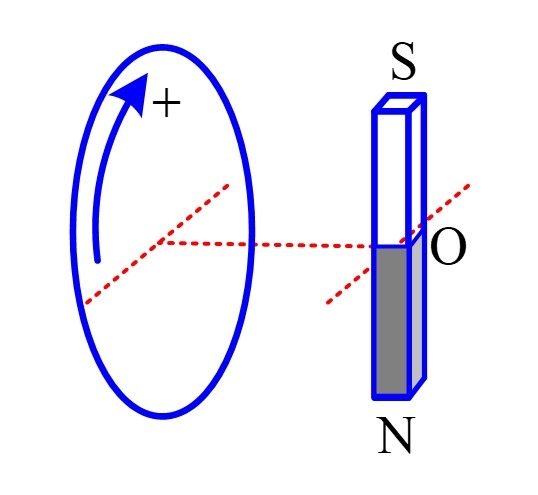
\includegraphics[scale=0.35]{../figs/VN11-PH-29-P-0191-4}
		\end{center}
		\begin{mcq}(1)
			\item{không có dòng điện cảm ứng.}
			\item{có dòng điện cảm ứng chạy theo chiều dương.}
			\item{có dòng điện cảm ứng chạy theo chiều âm.}
			\item{có dòng điện cảm ứng với cường độ biến thiên tuần hoàn theo thời gian.}
		\end{mcq}	
	}
	
	\loigiai{
		\textbf{Đáp án: C.}
		
		
	}
	\item \mkstar{2} 
	
	\cauhoi{
		Một khung dây dẫn tròn, nhẹ, được treo bằng sợi dây mềm, đường thẳng $x'x$ trùng với trục của khung dây, một nam châm thẳng đặt dọc theo trục $x'x$, cực Bắc của nam châm gần khung dây như hình vẽ. Tịnh tiến nam châm
		\begin{center}
			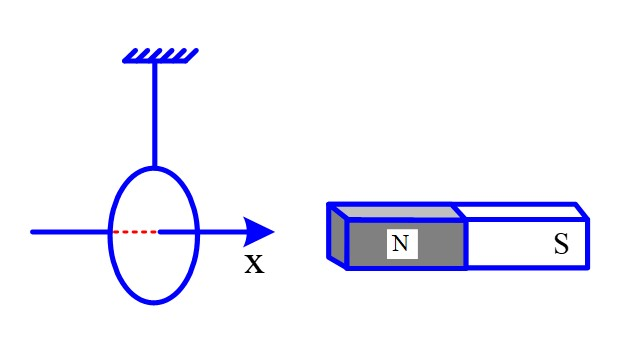
\includegraphics[scale=0.4]{../figs/VN11-PH-29-P-0191-5}
		\end{center}
		\begin{mcq}(1)
			\item{lại gần khung dây thì thấy khung dây chuyển động theo chiều dương trục $x'x$.}
			\item{lại gần khung dây thì thấy khung dây chuyển động theo chiều âm trục $x'x$.}
			\item{ra xa khung dây thì thấy khung dây chuyển động theo chiều âm trục $x'x$.}
			\item{thì chúng luôn đẩy khung dây.}
		\end{mcq}
	}
	
	\loigiai{
		\textbf{Đáp án: B.}
		
		
	}
	\item \mkstar{2} 
	
	\cauhoi{
		Một khung dây dẫn rất nhẹ được treo bằng sợi dây mềm, đường thẳng $x'x$ trùng với trục của khung dây. Khung dây được đặt gần một nam châm điện, trục nam châm điện trùng với trục $x'x$. Khi cho con chạy của biến trở dịch chuyển từ M đến N thì
		\begin{center}
			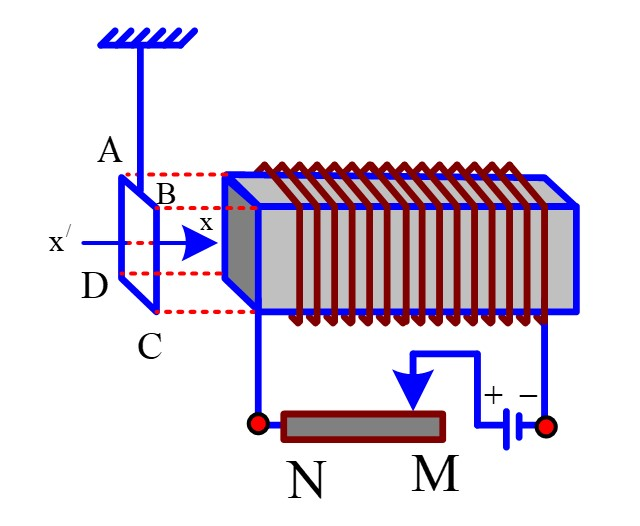
\includegraphics[scale=0.4]{../figs/VN11-PH-29-P-0191-6}
		\end{center}
		\begin{mcq}(1)
			\item{trong khung dây không có dòng điện cảm ứng.}
			\item{trong khung dây xuất hiện dòng điện cảm ứng có chiều ABCD.}
			\item{khung dây bị đẩy ra xa nam châm.}
			\item{khung dây bị hút lại gần nam châm.}
		\end{mcq}	
	}
	
	\loigiai{
		\textbf{Đáp án: C.}
		
		
	}
	\item \mkstar{2} 
	
	\cauhoi{
		Một khung dây dẫn tròn gồm $N$ vòng. Khung nằm trong từ trường đều, mặt phẳng khung song song với đường sức từ như hình vẽ. Cho khung quay xung quanh trục MN, qua tâm của khung và trùng với một đường sức từ thì
		\begin{center}
			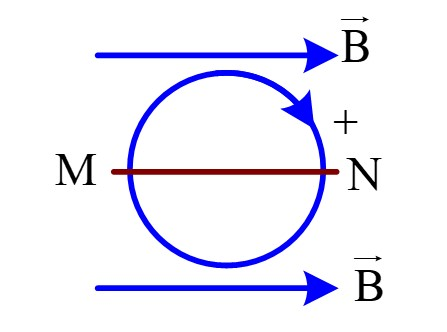
\includegraphics[scale=0.4]{../figs/VN11-PH-29-P-0191-7}
		\end{center}
		\begin{mcq}(1)
			\item{không có dòng điện cảm ứng.}
			\item{có dòng điện cảm ứng chạy theo chiều dương.}
			\item{có dòng điện cảm ứng chạy theo chiều âm.}
			\item{có dòng điện cảm ứng với cường độ biến thiên tuần hoàn theo thời gian.}
		\end{mcq}	
	}
	
	\loigiai{
		\textbf{Đáp án: A.}
		
		+ Lúc đầu vì B song song với mặt khung nên góc giữa B và pháp tuyến của khung là $90^\circ$ nên $\Phi = 0$
		
		+ Khi quay khung xung quanh trục MN như hình vẽ thì góc giữa B và pháp tuyến luôn là $90^\circ$.
		
		Suy ra không có dòng điện cảm ứng.
	}

		\item \mkstar{2} 
	
	\cauhoi{
		
		Cho dòng điện thẳng cường độ $I$ không đổi và khung dây dẫn hình chữ nhật MNPQ, cạnh MQ của khung sát với dòng điện như hình vẽ. Cho biết các dây dẫn đều có lớp vỏ cách điện. Cho khung dây dẫn quay xung quanh cạnh MQ của khung thì
		\begin{center}
			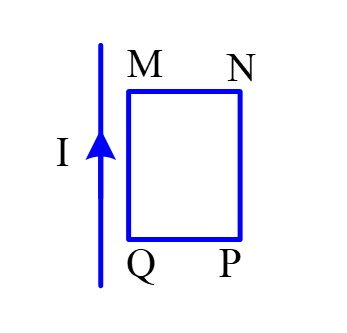
\includegraphics[scale=0.45]{../figs/VN11-PH-29-P-0191-8}
		\end{center}
		\begin{mcq}(1)
			\item{không có dòng điện cảm ứng.}
			\item{có dòng điện cảm ứng chạy theo chiều dương.}
			\item{có dòng điện cảm ứng chạy theo chiều âm.}
			\item{có dòng điện cảm ứng với cường độ biến thiên tuần hoàn theo thời gian.}
		\end{mcq}	
	}
	
	\loigiai{
		\textbf{Đáp án: A.}
		
		
	}
		\item \mkstar{2} 
	\cauhoi{
		
			Một vòng dây phẳng giới hạn diện tích $S=\SI{5}{\centi \meter \squared}$ đặt trong từ trường đều cảm ứng từ $B=\SI{0.1}{\tesla}$. Mặt phẳng vòng dây làm thành với từ trường một góc $\alpha = \ang{30}$. Tính từ thông qua $S$.
		\begin{mcq}(4)
			\item{$\SI{3e-4}{\weber}$.}
			\item{$\SI{3e-5}{\weber}$.}
			\item{$\SI{4.5e-5}{\weber}$.}
			\item{$\SI{2.5e-5}{\weber}$.}
		\end{mcq}	
	}
	
	\loigiai{
		\textbf{Đáp án: D.}
		
		Mặt phẳng vòng dây làm thành với B một góc $30^\circ$ nên $\alpha  = 60^\circ.$
		
		Từ thông qua $S$
		
		$$\Phi = BS \cos \alpha  = \SI{2.5e-5}{\weber}.$$
	}
		\item \mkstar{2} 
	\cauhoi{
		
		Một khung dây hình tròn đặt trong từ trường đều có cảm ứng từ $B=\SI{0.06}{\tesla}$ sao cho mặt phẳng khung dây vuông góc với các đường sức từ. Từ thông qua khung dây là $\SI{1.2e-5}{\weber}$. Bán kính vòng dây gần giá trị nào nhất sau đây?
		\begin{mcq}(4)
			\item{$\SI{12}{\milli \meter}$.}
			\item{$\SI{6}{\milli \meter}$.}
			\item{$\SI{7}{\milli \meter}$.}
			\item{$\SI{8}{\milli \meter}$.}
		\end{mcq}	
	}
	
	\loigiai{
		\textbf{Đáp án: D.}
		
		Bán kính vòng dây
		
		$$ R = \sqrt {\dfrac{\phi}{B \pi \cos \alpha}} = 8 \cdot 10^{-3}\ \text{m}.$$
	}
		\item \mkstar{2} 
	\cauhoi{
		
			Một khung dây phẳng giới hạn diện tích $S=\SI{5}{\centi \meter \squared}$ gồm 20 vòng dây đặt trong từ trường đều có cảm ứng từ $B=\SI{0.1}{\tesla}$ sao cho mặt phẳng khung dây hợp với vectơ cảm ứng từ một góc $\ang{60}$. Tính từ thông qua diện tích giới hạn bởi khung dây.
		\begin{mcq}(4)
			\item{$\SI{8.66e-4}{\weber}$.}
			\item{$\SI{5e-4}{\weber}$.}
			\item{$\SI{4.5e-5}{\weber}$.}
			\item{$\SI{2.5e-5}{\weber}$.}
		\end{mcq}	
	}
	
	\loigiai{
		\textbf{Đáp án: A.}
		
		Góc hợp bởi giữa pháp tuyển và cảm ứng từ $\alpha  = 30^\circ.$
		
		Từ thông qua diện tích $S$
		
		$$\Phi = NBS \cos \alpha  = \text{8,66} \cdot 10^{-4}\ \text{Wb}.$$
	}
		\item \mkstar{2} 
	\cauhoi{
		
		Một khung dây hình vuông cạnh $\SI{5}{\centi \meter}$ đặt trong từ trường đều có cảm ứng từ $B=\SI{8e-4}{\tesla}$. Từ thông qua hình vuông đó bằng $\SI{e-6}{\weber}$. Tính góc hợp giữa vectơ cảm ứng từ và vectơ pháp tuyến của hình vuông đó.
		\begin{mcq}(4)
			\item{$\alpha = \ang{0}$.}
			\item{$\alpha=\ang{30}$.}
			\item{$\alpha=\ang{60}$.}
			\item{$\alpha=\ang{90}$.}
		\end{mcq}	
	}
	
	\loigiai{
		\textbf{Đáp án: B.}
		
		Diện tích của khung
		
		$$S = a^2 = \text{2,5} \cdot 10^{-3}\ \text{m}^2.$$
		
		Góc hợp giữa vectơ cảm ứng từ và vectơ pháp tuyến 
		
		$$ \Phi = BS \cos \alpha \Rightarrow \alpha  = 60^\circ.$$
	}
		\item \mkstar{2} 
	\cauhoi{
		
		[Đề tham khảo của BGD-ĐT-2018] Một khung dây phẳng diện tích $\SI{20}{\centi \meter \squared}$ đặt trong từ trường đều có vectơ cảm ứng từ hợp với vectơ pháp tuyến của mặt phẳng khung dây một góc $\ang{60}$ và có độ lớn $\SI{0.12}{\tesla}$. Từ thông qua khung dây này là
		\begin{mcq}(4)
			\item{$\SI{2.4e-4}{\weber}$.}
			\item{$\SI{1.2e-4}{\weber}$.}
			\item{$\SI{1.2e-6}{\weber}$.}
			\item{$\SI{2.4e-6}{\weber}$.}
		\end{mcq}	
	}
	
	\loigiai{
		\textbf{Đáp án: B.}
		
		Từ thông qua khung dây:
		
		$$\Phi  = BS\cos \alpha  = \text{1,2} \cdot 10^{-4} \ \text{Wb}.$$
	}

\end{enumerate}
\section{Suất điện động cảm ứng}
\begin{enumerate}[label=\bfseries Câu \arabic*:]
	
	\item \mkstar{2} 
	
	\cauhoi{
		Cuộn dây có $N=100$ vòng, mỗi vòng có diện tích $S=\SI{300}{\centi \meter \squared}$, đặt trong từ trường đều có cảm ừng từ $B=\SI{0.2}{\tesla}$ sao cho trục của cuộn dây song song với các đường sức từ. Quay đều cuộn dây để sau $\Delta t= \SI{0.5}{\second}$ trục của nó vuông góc với các đường sức từ thì độ lớn suất điện động cảm ứng trung bình trong cuộn dây là
		\begin{mcq}(4)
			\item{$\SI{0.6}{\volt}$.}
			\item{$\SI{1.2}{\volt}$.}
			\item{$\SI{3.6}{\volt}$.}
			\item{$\SI{4.8}{\volt}$.}
		\end{mcq}
	}
	
	\loigiai{
		
		\textbf{Đáp án: B.}
		
		Suất điện động cảm ứng
		
		$$e_\text{c} = \left|\dfrac{\Delta \Phi}{\Delta t} \right| = \left|\dfrac{NBS (\cos \alpha_2 - \cos \alpha_1)}{\Delta t} \right| = \SI{1,2}{V}.$$
		
		
	}
	
	\item \mkstar{2}
	
	\cauhoi{
	Một khung dây có $100$ vòng được đặt trong từ trường đều sao cho các đường sức từ vuông góc với mặt phẳng của khung dây. Diện tích của mỗi vòng dây là $\SI{2}{\deci \meter \squared}$, cảm ứng từ giảm đều từ $\SI{0.5}{\tesla}$ đến $\SI{0.2}{\tesla}$ trong thời gian $\SI{0.1}{\second}$. Suất điện động cảm ứng trong khung dây là
	\begin{mcq}(4)
		\item{$\SI{6}{\volt}$.}
		\item{$\SI{60}{\volt}$.}
		\item{$\SI{3}{\volt}$.}
		\item{$\SI{30}{\volt}$.}
	\end{mcq}
	}
	\loigiai{
		
		\textbf{Đáp án: A.}
		
		Suất điện động cảm ứng trong khung dây
		
		$$e_\text c = \dfrac{\Delta \Phi}{\Delta t} = \dfrac{N \Delta B S \cos \alpha}{\Delta t} = \SI{6}{V}.$$
	}

	\item \mkstar{2} 
	
	\cauhoi{
		Một khung dây hình vuông có cạnh $\SI{5}{\centi \meter}$, đặt trong từ trường đều $\SI{0.08}{\tesla}$, mặt phẳng khung dây vuông góc với các đường sức từ. Trong thời gian $\SI{0.2}{\second}$, cảm ứng từ giảm xuống đến $0$. Độ lớn của suất điện động cảm ứng trong khung trong khoảng thời gian đó là
		\begin{mcq}(4)
			\item{$\SI{0.04}{\milli \volt}$.}
			\item{$\SI{0.5}{\milli \volt}$.}
			\item{$\SI{1}{\milli \volt}$.}
			\item{$\SI{8}{\volt}$.}
		\end{mcq}
	}
	
	\loigiai{
		\textbf{Đáp án: C.}
		
		Suất điện động cảm ứng
	
	$$e_\text{c} = \left|\dfrac{\Delta \Phi}{\Delta t} \right| = \left|\dfrac{BS \cos \alpha}{\Delta t} \right| = \SI{1}{mV}.$$
	}

		\item \mkstar{2} 
	
	\cauhoi{
		[Đề chính thức của BGD-ĐT-2018] Một vòng dây kín, phẳng được đặt trong từ trường đều. Trong khoảng thời gian $\SI{0.02}{\second}$, từ thông qua vòng dây giảm đều từ giá trị $\SI{4e-3}{\weber}$ về $0$ thì suất điện động cảm ứng xuất hiện trong vòng dây có độ lớn
		\begin{mcq}(4)
			\item{$\SI{0.2}{\volt}$.}
			\item{$\SI{8}{\volt}$.}
			\item{$\SI{2}{\volt}$.}
			\item{$\SI{0.8}{\volt}$.}
		\end{mcq}
		
	}
	\loigiai{
		
		\textbf{Đáp án: A.}
		
			Suất điện động cảm ứng
		
		$$e_\text{c} = \left|\dfrac{\Delta \Phi}{\Delta t} \right|  = \SI{0,2}{V}.$$
	}
		\item \mkstar{2} 
	
	\cauhoi{
		Thanh kim loại AB dài $\SI{20}{\centi \meter}$ kéo trượt đều trên hai thanh ray kim loại nằm ngang như hình vẽ.
		\begin{center}
			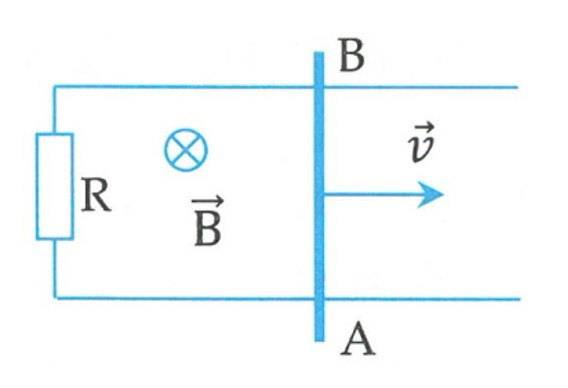
\includegraphics[scale=0.4]{../figs/VN11-PH-30-P-0201-1.jpg}
		\end{center}
		Các dây nối nhau bằng điện trở $R=\SI{3}{\Omega}$. Vận tốc của thanh AB là $\SI{12}{\meter / \second}$. Hệ thống đặt trong từ trường đều có $B=\SI{0.4}{\tesla}$, $\vec{B}$ vuông góc với mạch điện. Tìm suất điện động cảm ứng trong khung.
			\begin{mcq}(4)
				\item{$\SI{0.48}{\volt}$.}
				\item{$\SI{0.96}{\volt}$.}
				\item{$\SI{0.83}{\volt}$.}
				\item{$\SI{0.69}{\volt}$.}
			\end{mcq}
		
	}
	\loigiai{
		
		\textbf{Đáp án: B.}
		
		Suất điện động cảm ứng trong thanh
		
		$$e_\text c = Bvl \sin 90^\circ = \SI{0,96}{V}.$$ 
	}
	
	
\end{enumerate}

\section{Tự cảm}
\begin{enumerate}[label=\bfseries Câu \arabic*:]
	
	\item \mkstar{2} 
	
	\cauhoi{
		Ống dây điện hình trụ có chiều dài tăng gấp đôi (các đại lượng khác không thay đổi) thì độ tự cảm
	\begin{mcq}(2)
		\item {không đổi.}
		\item {tăng 4 lần.}
		\item {tăng 2 lần.}
		\item {giảm 2 lần.}
	\end{mcq}
	}
	
	\loigiai{
		\textbf{Đáp án: D.}
		
	Độ tự cảm của ống dây 
	
	$$ L =4\pi 10^{-7} \dfrac{N^2}{l}S.$$
	}
	
	\item \mkstar{2} 
	
	\cauhoi{
		Ống dây điện hình trụ có số vòng dây tăng 2 lần (các đại lượng khác không thay đổi) thì độ tự cảm
		\begin{mcq}(2)
			\item{tăng 2 lần.}
			\item{tăng 4 lần.}
			\item{giảm 2 lần.}
			\item{giảm 4 lần.}
		\end{mcq}
		
	}
	\loigiai{
		
		\textbf{Đáp án: B.}
		
		Độ tự cảm của ống dây 
	
	$$ L =4\pi 10^{-7} \dfrac{N^2}{l}S.$$
	}
	
	\item \mkstar{2}
	
	\cauhoi{
		Ống dây điện hình trụ có số vòng dây tăng 4 lần và chiều dài tăng 2 lần (các đại lượng khác không thay đổi) thì độ tự cảm
		\begin{mcq}(2)
			\item{tăng 8 lần.}
			\item{tăng 4 lần.}
			\item{giảm 2 lần.}
			\item{giảm 4 lần.}
		\end{mcq}
		
	}
	\loigiai{
		
		\textbf{Đáp án: A.}
	
	Độ tự cảm của ống dây 
	
	$$ L =4\pi 10^{-7} \dfrac{N^2}{l}S.$$
	}

		\item \mkstar{2} 
	
	\cauhoi{
	Tính độ tự cảm của một ống dây hình trụ có chiều dài $\SI{0.5}{\meter}$ gồm $1000$ vòng dây, mỗi vòng dây có đường kính $\SI{20}{\centi \meter}$.
	\begin{mcq}(4)
		\item{$\SI{0.088}{\henry}$.}
		\item{$\SI{0.079}{\henry}$.}
		\item{$\SI{0.125}{\henry}$.}
		\item{$\SI{0.064}{\henry}$.}
	\end{mcq}	
		
	}
	\loigiai{
		
		\textbf{Đáp án: B.}
	
	Độ tự cảm của ống dây 
	
	$$ L =4\pi 10^{-7} \dfrac{N^2}{l}S=\SI{0.079}{\henry}.$$
	}
	
		\item \mkstar{2} 
	
	\cauhoi{
		[Đề chính thức của BGD-ĐT-2018] Một cuộn cảm có độ tự cảm $\SI{0.2}{\henry}$. Trong khoảng thời gian $\SI{0.05}{\second}$, dòng điện trong cuộn cảm có cường độ giảm đều từ $\SI{2}{\ampere}$ xuống $0$ thì suất điện động tự cảm xuất hiện trong cuộn cảm có độ lớn là
		\begin{mcq}(4)
			\item{$\SI{4}{\volt}$.}
			\item{$\SI{0.4}{\volt}$.}
			\item{$\SI{0.02}{\volt}$.}
			\item{$\SI{8}{\volt}$.}
		\end{mcq}
		
	}
	\loigiai{
		
		\textbf{Đáp án: D.}
		
		Suất điện động tự cảm
		
		$$|e_\text{tc} |= L \dfrac{|\Delta i|}{\Delta t} = \SI{8}{V}.$$
	}
	
		\item \mkstar{2} 
	
	\cauhoi{
		Một cuộn cảm có độ tự cảm $\SI{0.5}{\henry}$, trong đó dòng điện tăng đều với tốc độ $\SI{200}{\ampere / \second}$ thì suất điện động tự cảm là
		\begin{mcq}(4)
			\item{$\SI{-100}{\volt}$.}
			\item{$\SI{20}{\volt}$.}
			\item{$\SI{100}{\volt}$.}
			\item{$\SI{200}{\volt}$.}
		\end{mcq}
		
	}
	\loigiai{
		
		\textbf{Đáp án: A.}
		
			Suất điện động tự cảm
		
		$$e_\text{tc} = - L \dfrac{\Delta i}{\Delta t} = -\SI{100}{V}.$$
	}
	
		\item \mkstar{2} 
	
	\cauhoi{
			Dòng điện qua một ống dây không có lõi sắt biến đổi theo thời gian. Trong thời gian $\SI{0.01}{\second}$ cường độ dòng điện tăng từ $i_1=\SI{1}{\ampere}$ đến $i_2=\SI{2}{\ampere}$, suất điện động tự cảm trong ống dây có độ lớn bằng $\SI{20}{\volt}$. Hệ số tự cảm của ống dây là
		\begin{mcq}(4)
			\item{$\SI{0.1}{\henry}$.}
			\item{$\SI{0.4}{\henry}$.}
			\item{$\SI{0.2}{\henry}$.}
			\item{$\SI{0.6}{\henry}$.}
		\end{mcq}
		
	}
	\loigiai{
		
		\textbf{Đáp án: C.}
		
		
		Hệ số tự cảm của ống dây
		
		$$ L  = \dfrac{|e_\text{tc}|\Delta t}{|\Delta i|} =\SI{0,2}{H}.$$
	}
	
		\item \mkstar{2}
	
	\cauhoi{
	Suất điện động tự cảm $\SI{0.75}{\volt}$ xuất hiện trong một cuộn cảm có $L=\SI{25}{\milli \henry}$, tại đó cường độ dòng điện giảm từ giá trị $I$ xuống $0$ trong $\SI{0.01}{\second}$. Tính $I$.
	\begin{mcq}(4)
		\item{$\SI{0.1}{\ampere}$.}
		\item{$\SI{0.4}{\ampere}$.}
		\item{$\SI{0.3}{\ampere}$.}
		\item{$\SI{0.6}{\ampere}$.}
	\end{mcq}
		
	}
	\loigiai{
		
		\textbf{Đáp án: C.}
		
		Cường độ dòng điện
		
		$$I = \dfrac{|e_\text{tc}| \Delta t}{L} = \SI{0,3}{A}.$$ 
	}
	
		\item \mkstar{2}
	
	\cauhoi{
			Trong một mạch kín có độ tự cảm $\SI{0.5e-3}{\henry}$, nếu suất điện động tự cảm có độ lớn bằng $\SI{0.25}{\volt}$ thì tốc độ biến thiên của dòng điện là
		\begin{mcq}(4)
			\item{$\SI{250}{\ampere / \second}$.}
			\item{$\SI{400}{\ampere / \second}$.}
			\item{$\SI{600}{\ampere / \second}$.}
			\item{$\SI{500}{\ampere / \second}$.}
		\end{mcq}
		
	}
	\loigiai{
		
		\textbf{Đáp án: D.}
		
		Tốc độ biến thiên của dòng điện
		
		$$\left|\dfrac{\Delta i}{\Delta r}\right| = \dfrac{|e_\text{tc}|}{L} = \SI{500}{\ampere / \second}.$$
	}
	
		\item \mkstar{2} 
	
	\cauhoi{
			Một ống dây dài $l=\SI{30}{\centi \meter}$ gồm $N=1000$ vòng dây, đường kính mỗi vòng dây $d=\SI{8}{\centi \meter}$ có dòng điện với cường độ $i=\SI{2}{\ampere}$ đi qua. Tính từ thông qua mỗi vòng dây
		\begin{mcq}(4)
			\item{$\SI{42}{\micro \weber}$.}
			\item{$\SI{0.4}{\micro \weber}$.}
			\item{$\SI{0.2}{\micro \weber}$.}
			\item{$\SI{86}{\micro \weber}$.}
		\end{mcq}
		
	}
	\loigiai{
		
		\textbf{Đáp án: B.}
		
		Từ thông qua ống dây
		
		$$ \Phi = L i = 4 \pi 10^{-7} \dfrac{N^2}{l} S i =\SI{0,04}{Wb}.$$
		
		Từ thông qua mỗi vòng dây
		
		$$ \phi = \dfrac{\Phi}{N} = 4 \cdot 10^{-5}\ \text{Wb}.$$
	}
	
		\item \mkstar{2} 
	
	\cauhoi{
		Một ống dây dài $l=\SI{30}{\centi \meter}$ gồm $N=1000$ vòng dây, đường kính mỗi vòng dây $d=\SI{8}{\centi \meter}$ có dòng điện với cường độ $i=\SI{2}{\ampere}$ đi qua. Thời gian ngắt dòng điện là $t=\SI{0.1}{\second}$, độ lớn suất điện động tự cảm xuất hiện trong ống dây là
		\begin{mcq}(4)
			\item{$\SI{0.15}{\volt}$.}
			\item{$\SI{0.42}{\volt}$.}
			\item{$\SI{0.24}{\volt}$.}
			\item{$\SI{8.6}{\volt}$.}
		\end{mcq}
		
	}
	\loigiai{
		
		\textbf{Đáp án: B.}
		
		Suất điện động tự cảm
		
		$$|e_\text{tc} |=  \left|- 4 \pi 10^{-7} \dfrac{N^2}{l} S \dfrac{\Delta i}{\Delta t}\right| = \SI{0,42}{V}.$$
	}
	
\end{enumerate}	
\whiteBGstarEnd